\documentclass[paper=a4, fontsize=11pt]{scrartcl} % A4 paper and 11pt font size

\newcommand{\assignment}{3}
\newcommand{\duedate}{February 15, 2023}
\usepackage[top=1in, bottom=1.5in, left=1in, right=1in]{geometry}
\usepackage{fancyhdr} % Required for custom headers
\usepackage{lastpage} % Required to determine the last page for the footer
\usepackage{extramarks} % Required for headers and footers
\usepackage[usenames,dvipsnames]{color} % Required for custom colors
\usepackage{graphicx} % Required to insert images
\usepackage{listings} % Required for insertion of code
\usepackage{courier} % Required for the courier font
\usepackage{amsmath}
\usepackage[super]{nth}
\usepackage{booktabs}
\usepackage[usenames,dvipsnames]{xcolor}
\usepackage{tcolorbox}
\usepackage{tabularx}
\usepackage{array}
\usepackage{colortbl}

%\usepackage[T1]{fontenc} % Use 8-bit encoding that has 256 glyphs
%\usepackage{fourier} % Use the Adobe Utopia font for the document - comment this line to return to the LaTeX default
\usepackage[english]{babel} % English language/hyphenation
\usepackage{amsmath,amsfonts,amsthm} % Math packages
\usepackage{graphicx}

\usepackage{hyperref}
\hypersetup{
  colorlinks   = true, %Colours links instead of ugly boxes
  urlcolor     = blue, %Colour for external hyperlinks
  linkcolor    = blue, %Colour of internal links
  citecolor   = red %Colour of citations
}

\usepackage{fancyhdr} % Custom headers and footers
\pagestyle{fancyplain} % Makes all pages in the document conform to the custom headers and footers
\fancyhead{} % No page header - if you want one, create it in the same way as the footers below
\fancyfoot[L]{} % Empty left footer
\fancyfoot[C]{} % Empty center footer
\fancyfoot[R]{\thepage} % Page numbering for right footer
\renewcommand{\headrulewidth}{0pt} % Remove header underlines
\renewcommand{\footrulewidth}{0pt} % Remove footer underlines
\setlength{\headheight}{13.6pt} % Customize the height of the header
\newcommand{\ts}{\textsuperscript}

\numberwithin{equation}{section} % Number equations within sections (i.e. 1.1, 1.2, 2.1, 2.2 instead of 1, 2, 3, 4)
\numberwithin{figure}{section} % Number figures within sections (i.e. 1.1, 1.2, 2.1, 2.2 instead of 1, 2, 3, 4)
\numberwithin{table}{section} % Number tables within sections (i.e. 1.1, 1.2, 2.1, 2.2 instead of 1, 2, 3, 4)

\setlength\parindent{0pt} % Removes all indentation from paragraphs - comment this line for an assignment with lots of text

% Default fixed font does not support bold face
\DeclareFixedFont{\ttb}{T1}{txtt}{bx}{n}{8} % for bold
\DeclareFixedFont{\ttm}{T1}{txtt}{m}{n}{8}  % for normal

%----------------------------------------------------------------------------------------
%	CODE BLOCKS
%----------------------------------------------------------------------------------------

\usepackage{adjustbox}
\usepackage{listings}
\usepackage{color}

\definecolor{dkgreen}{rgb}{0,0.6,0}
\definecolor{gray}{rgb}{0.5,0.5,0.5}
\definecolor{mauve}{rgb}{0.58,0,0.82}

\lstdefinelanguage{Dockerfile}
{
  morekeywords={FROM, RUN, CMD, LABEL, MAINTAINER, EXPOSE, ENV, ADD, COPY,
    ENTRYPOINT, VOLUME, USER, WORKDIR, ARG, ONBUILD, STOPSIGNAL, HEALTHCHECK,
    SHELL},
  morecomment=[l]{\#},
  morestring=[b]"
}

\lstset{
    columns=flexible,
    aboveskip=5mm,
    belowskip=5mm,
    keepspaces=true,
    showstringspaces=false,
    basicstyle=\ttfamily,
    commentstyle=\color{gray},
    keywordstyle=\color{purple},
    stringstyle=\color{green}
}



%----------------------------------------------------------------------------------------
%	TITLE SECTION
%----------------------------------------------------------------------------------------

\usepackage{eso-pic}
% \usepackage[demo]{graphicx}
\newcommand\AtPageUpperRight[1]{\AtPageUpperLeft{%
   \makebox[\paperwidth][r]{#1}}}

\newcommand{\horrule}[1]{\rule{\linewidth}{#1}} % Create horizontal rule command with 1 argument of height

\title{	
\normalfont \normalsize
\textsc{Northeastern University,  Khoury College of Computer Science} \\ [25pt] % Your university, school and/or department name(s)
\horrule{0.5pt} \\[0.4cm] % Thin top horizontal rule
\huge CS 6220  Data Mining \textemdash~Assignment \assignment \\ % The assignment title
\Large \textbf{Due: \duedate (100 points)} % The assignment title
\horrule{2pt} \\[0.5cm] % Thick bottom horizontal rule
}

% Original in the document
\AddToShipoutPictureBG*{%
  \AtPageUpperRight{\raisebox{-\height}{
\includegraphics[width=3cm]{images/logo}}}}

\author{
    \textbf{YOUR NAME} \\ 
    \textbf{YOUR GIT USERNAME} \\ 
    \textbf{YOUR E-MAIL}
}% INFORMATION

\date{} % Today's date or a custom date
\author{
    \textbf{YOUR NAME} \\ 
    \textbf{YOUR GIT USERNAME} \\ 
    \textbf{YOUR E-MAIL}
}% INFORMATION

\begin{document}

\maketitle % Print the title

{\huge \textbf{Multisource Joins}}  \\

News articles are commonly aggregated from multiple sites and companies. The landscape of news has been evolving ever since social media has amplified its effects. In politics, Congress has explored the topic of bias with the diversity of news sources. That is, news articles may cover news stories with differing perspectives and language. \\

The data that we will be using today comes from Kaggle, and it is available \href{https://course.ccs.neu.edu/cs6220/homework-3/}{here}. There are two CSV files that we wish to join in this week's homework:

\begin{itemize}
    \item \verb"data/id_titles.csv"
    \item \verb"data/id_publishers.csv"
\end{itemize}

As there name suggests, there is publishing data associated with articles and there is title and description information associated with the same articles. Each table has many instances, and each instance for both tables have an associated ID, where it is possible to join the two data sources.

In this particular case, there is some missing information in the join. Your task is as follows. \\

\textbf{Question 1 a.)}
\begin{itemize}
    \item Write out a file that has all the publishers for which there are no titles, called publishers\_no\_titles.txt. This table should look something like the below (ignore the values): \\
    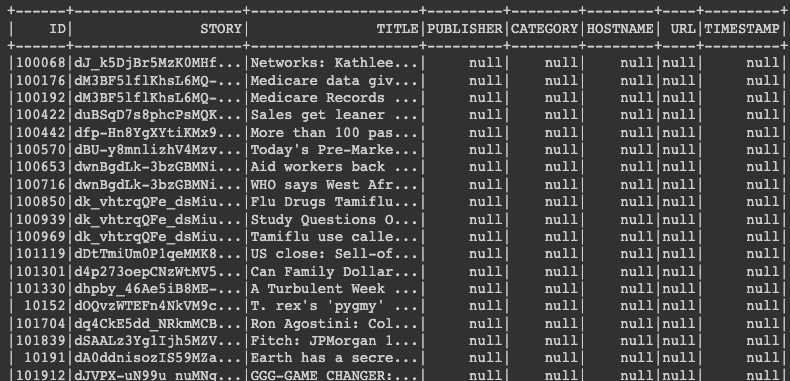
\includegraphics[width=100mm]{images/pub_no_title.png}
\end{itemize} \\

\textbf{Question 1 b.)}
\begin{itemize}
    \item Write out a file that has all the publishers for which there are no titles, called titles\_no\_publishers.txt. That table should look something like the below (ignore the values): \\
    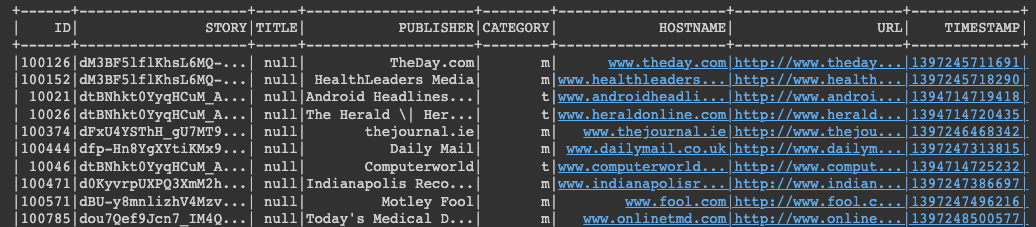
\includegraphics[width=150mm]{images/title_no_pub.png}
\end{itemize} \\
\\
.\\
\\
{\huge \textbf{Frequent Itemsets}} \\
%%%%%%%%%%%%%%%%%%%%

Consider the following set of frequent 3-itemsets:

\begin{verbatim}
{1, 2, 3}, {1, 2, 4}, {1, 2, 5}, {1, 3, 4}, 
{2, 3, 4}, {2, 3, 5}, {3, 4, 5}.
\end{verbatim} \\

Assume that there are only five items in the data set. \\

{\Large \textbf{Question 2} [15 pts total]} \\
\\
\textbf{[5 pts] Question 2a.)} List all candidate 4-itemsets obtained by a candidate generation procedure using the $F_{k - 1} \times F_1$ merging strategy. \\
\\
\textbf{[5 pts] Question 2b.)} List all candidate 4-itemsets obtained by the candidate generation procedure in A Priori, using $F_{k-1} \times F_{k-1}$. \\
\\
\textbf{[5 pts] Question 2c.)} List all candidate 4-itemsets that survive the candidate pruning step of
the Apriori algorithm. \\
\\
\\
{\huge \textbf{Parameter Estimation}} \\

It is well-known that light bulbs commonly go out according to a Poisson distribution, and are independent regardless of whether or not they're made in the same factory. An architect has outfitted a building with 32,000 of the same lightbulb. \\
\\
{\Large \textbf{Question 3} [15 pts total]} \\
\\
Assuming the Poisson distribution has the form:
\begin{equation}
p(X | \lambda) = \frac{ \exp^{-\lambda} \lambda ^{x_i}}{ x_i !}
\end{equation}
derive the maximum likelihood estimate of the parameter $\lambda$ in terms of $x_i$. \\
\\


%%%%%%%%%%%%%%%%%%%%
{\huge \textbf{Submission Instructions}} \\
%%%%%%%%%%%%%%%%%%%%

When you have finished, follow the instructions on the \href{https://course.ccs.neu.edu/cs6220/homework-3/}{ homework main page} commit your code, outputs, and PDF writeup to your repository and provide the repository link to \href{https://www.gradescope.com}{Gradescope}.


\end{document}
